% -------------------------------------------------------------------------------------------------
%      MDSG Latex Framework
%      ============================================================================================
%      File:                  introduction-[UTF8,ISO8859-1].tex
%      Author(s):             Michael Duerr
%      Version:               1
%      Creation Date:         30. Mai 2010
%      Creation Date:         30. Mai 2010
%
%      Notes:                 - Example chapter
% -------------------------------------------------------------------------------------------------
%
\chapter{Results}\label{sec:Results}
% - Result presentation
% - Description of images and charts \\
% - One Agent Environment vs MARL
% - Best cases of reward, trades, grid coloration, field resets
% - Worst cases of above
% - influence of markets
In this chapter the results of various training executions with different parameters are compared. All possible combinations of markets, agent compositions and learning algorithms in an easy environment are shown in section \ref{easy_env}. The best combinations are then extracted and applied in more challenging environment setups, which are compared in section \ref{difficult_env}. 

\section{Easy Environment Setup} \label{easy_env}
\marginpar{was wurde untersucht}
The results of this research compare multiagent trainings with varying settings, namely acting in different compositions and markets. In this case the amount of agents stays fixed and is greater than one. The agents use either of the two learning approaches PPO or DQN to train. Hence, the overall possible comparisons include a total amount of 102 executions. This number results from the calculation of multiplying the 2 learning algorithms with the 3 possible agent compositions (cooperative, competitive and mixed-motive) and additionally 2 optional markets that can contain 3 modular additions. 

The market options are for example the following SM instances: 
\begin{itemize}
    \item ``sm''
    \item ``sm-goal''
    \item ``sm-no-debt''
    \item ``sm-no-reset''
    \item ``sm-no-reset-no-debt''
    \item ``sm-goal-no-debt''
    \item ``sm-goal-no-reset''
    \item ``sm-goal-no-reset-no-debt''
\end{itemize}
The 8 options above are also applied on the AM and lastly the option of no market needs to be considered, leading to 17 market scenarios. Calculating the total amount of executions now by using those 17 market possibilities results in the 102 executions.

\marginpar{was wurde nicht untersucht}
Yet, not all market arrangements are needed. For example, the mix of ``no-reset'' and ``no-debt'' is not of use in this implementation. An agent that has reset a field has a reward of -0.1 and therefore already is in debt, which means that ``no-debt'' includes ``no-reset''. This subtracts 4 compositions from the 17 market scenarios. Additionally, shares are free of charge, making the options ``sm-no-debt'' and ``sm-goal-no-debt'' irrelevant. Agents can always afford to buy shares in this case. The SM is therefore left with 4 combinations and the overall market scenario count is now 11. In total the analyzation only includes 66 training results. 

\marginpar{wie wurde untersucht / zahlen}
In order to compare the market approach with a credit assignment solution in the cooperation composition, the training with a DR setting is also included. This in turn adds another execution to each learning algorithm. Furthermore, to ensure that the environment is generally solvable, one agent first trains in the environment setup with each learning algorithm using similar hyperparameter as in the multiagent case. To summarize the execution count is therefore 70 in total.

Those 70 executions are mostly run with the default parameters that can be looked up in Appendix \ref{ax:training_params}. The agents solve an empty 5 by 5 grid, in which they can only walk inside a 3 by 3 field, due to the surrounding walls, see Figure \ref{fig:1-easy}. The maximum amount of steps the agents are allowed to take is set to 25, if not specified otherwise. This count is generated by squaring the grid size.

Overall the training with default parameters expands over 80.000 frames, of which every 128 (\verb|--frames-per-proc|) are processed in each of the parallel environments. In this case the amount of parallel environments is set to 16 with the parameter \verb|--procs|. All the data that is returned by the environments is saved in one entry. Most of the time the data is summarized into mean values or occurrences are counted. Furthermore, the data entries are always 2048 frames apart, since all 16 environments process 128 actions before a new data entry is logged. After saving each entry the variables containing mean values or counters are reset to produce new values in the next frames. \\\\

% Those data entries 2048 frames are referred to as a batch. After each data batch, mean values and counters of all finished episodes are calculated and logged, for example mean rewards, mean grid coloration, amount of goal states or reset fields etc... 
% In the worst case scenario, where the episode always ended because the 25 default steps were used up, the data entry would contain values of 80 episodes. This is result of 25 fully executed steps in a span of 128 frames, leading to 5 finished episodes. This is the case for each of the 16 parallel environments. Afterwards, After each entry, all log variables are cleared to produce new values in the next frames. All environment data are put together to either calculate mean values or count occurrences.

% ------------ ONE AGENT RESULTS ----------------
\begin{minipage}{\textwidth}
  \begin{minipage}[b]{0.29\textwidth}
    \centering
    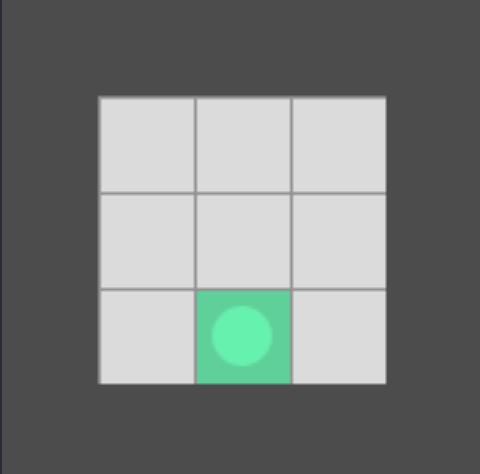
\includegraphics[width=1\linewidth]{1-agent-easy.png}\\
    \captionof{figure}[One Agent Level Easy]{Visualization of level easy with one agent}\label{fig:1-easy}
  \end{minipage}
  \hfill
  \begin{minipage}[b]{0.69\textwidth}
    \centering
    \begin{tabular}{lc}\hline
      Setting & Fully colored \\ \hline
        1 ppo & 2130 \\
        1 dqn & 650 \\ \hline
      \end{tabular}
      \captionof{table}[Training Results for one Agent Level Easy]{Number of times the agent fully colored the environment during training with each learning algorithm.}\label{t:1-easy}
    \end{minipage}
  \end{minipage}\\\\

Table \ref{t:1-easy} shows the amount of times the grid on the left (Figure \ref{fig:1-easy}) was fully colored by one agent using each training algorithm. It is important to mention here, that the maximum step amount is set to 10 in both cases. Additionally, this and all following dqn executions have a \verb|--batch-size| set to 64 instead of the default 256. The ppo agent colored the whole grid a total amount of 2130 times and the dqn agent 650 times.

\begin{figure}[hpbt]
    \centering
    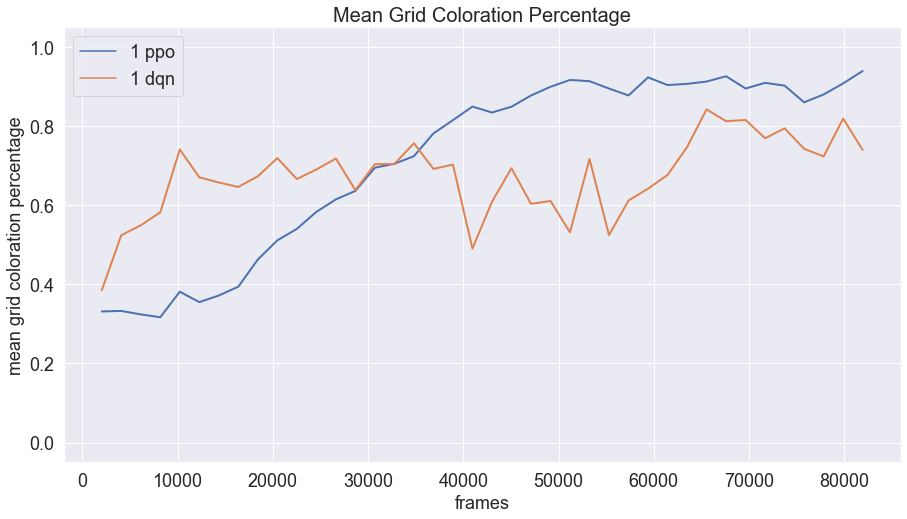
\includegraphics[width=0.8\textwidth]{1-easy-plot.png}\\
    \caption[Mean Grid Coloration Percentage of one Agent]{The mean coloration percentage of a 5x5 grid and one acting agent}\label{fig:1-easy-plot}
\end{figure}

The average grid coloration percentage of those settings is shown in plot \ref{fig:1-easy-plot}. The plot lines start at around 2048 frames, since this marks the first time a data entry of the parallel environments is returned. Furthermore, the plot exceeds the 80.000 default \verb|--frames|, since the last data entry includes the last data batch of the environments. The table shows, that both training runs solve the environment and the plot illustrates that in both cases generally a high percentage of the grid is colored. The dqn execution yields a better performance in the early stage, whereas the ppo agent gradually improves over time. In both cases an average coloration of over 70\% is eventually reached. 

Now the multiagent scenario is compared. Here a set of two agents are trained to color the field of the same default dimensions, see Figure \ref{fig:2-coop-easy}. However, every agent executes an action during a step and with 10 steps and two agents in theory 20 cells could be visited. Hence, the \verb|--max-steps| count is reduced to 8. 

In order to get an overview of the overall 70 training results, the remaining 68 multiagent executions are divided into three different \verb|--setting| values. The first data division only covers the cooperation compositions, including ``difference-reward''. Table \ref{t:2-coop-easy} illustrates the scoreboard of the top three executions in this specification for each learning algorithm. \\\\

% ------------ COOP RESULTS ----------------
\begin{minipage}{\textwidth}
  \begin{minipage}[b]{0.29\textwidth}
    \centering
    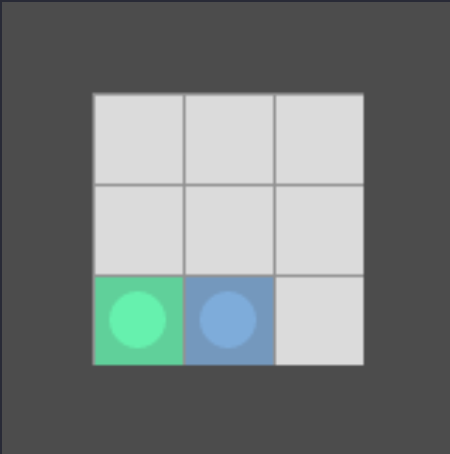
\includegraphics[width=1\linewidth]{2-agents-easy.png}\\
    \captionof{figure}[Two Agents Level Easy]{Visualization of level easy with two agents}\label{fig:2-coop-easy}
  \end{minipage}
  \hfill
    \begin{minipage}[b]{0.69\textwidth}
    \centering
    \begin{tabular}{lc}\hline
        Top 3 PPO Cooperation Settings & Fully colored \\ \hline
        2 ppo difference-reward & 889 \\
        2 ppo & 125 \\
        2 ppo sm-goal & 32 \\ \hline
         &   \\ \hline
        Top 3 DQN Cooperation Settings & Fully colored \\ \hline
        2 dqn difference-reward & 5949 \\
        2 dqn am-goal-no-debt & 3197 \\
        2 dqn am-goal & 2880 \\ \hline
        \end{tabular}
        \captionof{table}[Training Results for two Cooperation Agents Level Easy]{Number of times two agents working in cooperation fully colored the environment during training.}\label{t:2-coop-easy}
    \end{minipage}
  \end{minipage}\\\\

The measured attribute here is again the overall amount of fully colored states. In both cases the agents with the DR setting scored best, 889 times with the DQN algorithm and 5949 times by using PPO. The PPO scores continue with the default cooperation scenario on second and the SM with the goal condition on third place. 

On the contrary, the DQN results show AM settings on the remaining places, with the additions ``goal-no-reset'' on second place and ``goal'' on the third place. It is visible, that in both scoreboards the second and third executions are far behind the corresponding DR setting in terms of fully coloration counts.

\begin{figure}[hpbt]
    \centering
    %%----start of first subfigure----
    \subfloat[Reward summary of PPO agents]{
        \label{fig:2-ppo-coop-easy} %% label for first subfigure
        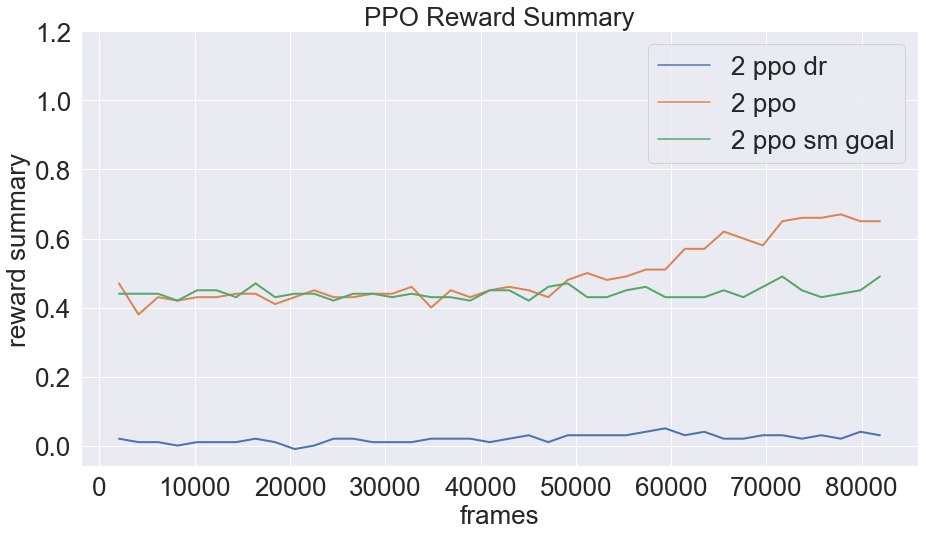
\includegraphics[width=0.48\linewidth]{2-ppo-easy.png}}
    \hspace{0.01\textwidth}
    %%----start of second subfigure----
    \subfloat[Reward summary of DQN agents]{
        \label{fig:2-dqn-coop-easy} %% label for second subfigure
        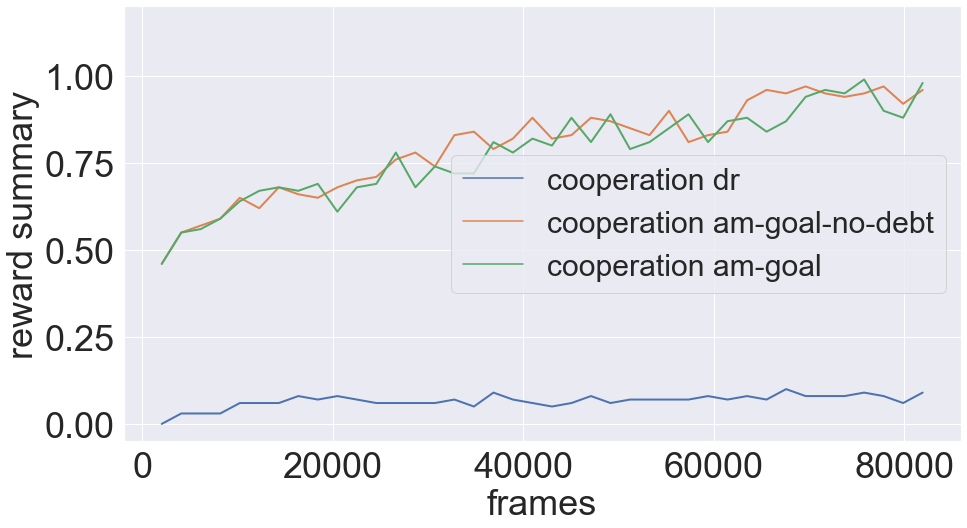
\includegraphics[width=0.48\linewidth]{2-dqn-easy.png}}
    \caption[Reward Summaries of the Top Cooperation Modes]{Reward Summaries of the top three cooperation compositions using PPO (left) and DQN (right)}
    \label{fig:multipic_plots_coop_easy} %% label for entire figure
\end{figure}

In the two plots of Figure \ref{fig:multipic_plots_coop_easy} the reward summary of the top scores, see table \ref{t:2-coop-easy}, are displayed. The term reward summary is used here, since the rewards of cooperating agents are equal and sometimes contain only slight changes through markets. However, in other agent compositions the rewards are rather specific to each agents' contribution. In any case the logged training data contains the mean reward of every agent separately. 

In order to summarize cooperation rewards, the average value of those separate agent rewards is calculated for each data entry and the results are then plotted here. For reward summaries of all other compositions each data entry is summarized with the sum of the separate agent rewards. The maximum y-axis label here is set to 1.2, since agents can get a reward of 1.1 if they color the whole field and additionally get a reward of 0.1 for the final step. Through the reward summary calculations rounding errors may occur, which could in turn exceed the maximum reward of 1.1. Furthermore, markets could also contribute to bigger rewards. 

Even thought, the executions with the DR configuration scored highest in terms of reaching the goal, the reward line in this case stays around 0.1. The reason for that is, that agents get the difference of two rewards, leading to very small values. The rewards of the dqn executions show a continuous increase and almost exceed an average summary reward of 1. On the contrary, the ppo executions, excluding the DR setting, only show a small reward increase at the last third half of the training. The DR execution shows now striking changes here.

The next training executions to look at are ``mixed-motive'' settings. Here again a scoreboard, listing the top three results of each learning algorithm, is shown in table \ref{t:2-mixed-easy}.
% ------------ MIXED RESULTS ----------------
\begin{center}
    \begin{tabular}{lc}\hline
        Top 3 PPO Mixed-Motive Settings & Fully colored \\ \hline
        2 ppo mixed-motive & 1006 \\
        2 ppo mixed-motive sm-no-reset & 764 \\
        2 ppo mixed-motive sm & 680 \\ \hline
         &   \\ \hline
        Top 3 DQN Mixed-Motive Settings & Fully colored \\ \hline
        2 dqn mixed-motive sm & 5417 \\
        2 dqn mixed-motive am-no-reset & 5379 \\
        2 dqn mixed-motive sm-goal & 5302 \\ \hline
        \end{tabular}
        \captionof{table}[Training Results for two Mixed-Motive Agents Level Easy]{Number of times two agents working in a mixed-motive setting fully colored the environment during training.}\label{t:2-mixed-easy}
    \end{center}

While the default SM configuration occupies the first place of the DQN scoreboard, in the PPO board it is only on the third place. In fact, the first place of the ppo training is the plain ``mixed-motive'' setting without any additions. On the second place here is a SM training with the ``no-reset'' condition. The fully colored counts are very similar between the PPO trainings. The same applies to the values of the DQN board. The second place here is also occupied by a ``no-reset'' addition, however in this case it is applied to an AM. On the third place of the DQN executions is a SM with the ``goal'' addition.


% ------------ COMP RESULTS ----------------
\begin{center}
    \begin{tabular}{lc}\hline
        Top 3 PPO Competitive Settings & Fully colored \\ \hline
        2 ppo competitive & 3178 \\
        2 ppo competitive sm-no-reset & 2645 \\
        2 ppo competitive sm & 2437 \\ \hline
         &   \\ \hline
        Top 3 DQN Competitive Settings & Fully colored \\ \hline
        2 dqn competitive sm-goal-no-reset & 7877 \\
        2 dqn competitive sm & 7842 \\
        2 dqn competitive am-goal-no-debt & 7560 \\ \hline
        \end{tabular}
        \captionof{table}[Training Results for two Competitive Agents Level Easy]{Number of times two agents working in a competitive setting fully colored the environment during training.}\label{t:2-comp-easy}
    \end{center}


\section{Difficult Environment Setup} \label{difficult_env}